\documentclass[12pt]{article}
\usepackage{graphicx}
\usepackage{Style-Thesis-Report}
\usepackage{fancyvrb}
\usepackage{moreverb}
\usepackage{fullpage} % Package to use full page
\usepackage{wrapfig}
\edef\restoreparindent{\parindent=\the\parindent\relax}
\usepackage{parskip}
\restoreparindent

\usepackage{caption}
%   \captionsetup{format=hang}
\usepackage{tikz} 
\usepackage{amsmath}
\usepackage{amsthm}
\usepackage{hyperref}
\usepackage[normalem]{ulem} 
\usepackage{authblk}
\usepackage{amsfonts}
\usepackage{tabularx}
\usepackage{mathrsfs}
\usepackage{csquotes}
\usepackage{amssymb}
\usepackage{titling}
\usepackage{relsize}

\newtheorem{defn}{Definition}
\newtheorem*{exmp}{Example} 
\newtheorem{prpn}{Proposition}
\newtheorem{lemma}{Lemma}
\newtheorem*{corly}{Corollary}
\newtheorem*{pf}{Proof}
\newtheorem*{conj}{Conjecture}
  
\begin{document} 
	
\begin{titlepage} 
\thispagestyle{empty}
	\begin{center}
\Large
\textsc{The necessity of the reprioritization  of corporate governance goals in shareholder-centered countries}
		\large
		\vspace{1cm}
		
		Daniel J. Hutama
		\vspace{0.5 cm}
		
		December 20, 2016
        
        \vspace{0.5 cm}
	\end{center}
		\hrule
	\begin{abstract} 
This paper is concerned with the difficulty in enacting a countervailing power in countries that adopt a shareholder-centered governance model. In particular, we argue that shareholder-centered governance contributes to a widening of income inequality. This inequality results in a momentum for economically powerful actors to acquire more wealth at the expense of the middle class and working class. Moreover, wealthy actors use their influence to prevent the appearance of a countervailing power. Without a countervailing power, the shareholder-centered corporation will ultimately be the cause of its own downfall. As a result, it is in the corporation's best interest to shift its focus to meet the needs of its stakeholders and work toward a reduction in inequality. Using the ratio of the average income of a country's richest $10\%$ to the poorest $10\%$ (denoted $10\% \text{ } R/P$), we found empirical evidence that income inequality at a national level may be linked to the country's corporate governance model. In particular, we found that countries following a German (stakeholder-centered) legal tradition have a $10\% \text{ } R/P$ of $6.9 \pm 1.5$, while countries following an Anglo-Saxon (shareholder-centered) legal tradition have a $10\% \text{ } R/P$ of $16.4 \pm 7.1$.


\end{abstract}
\hrule
\end{titlepage}
%\tableofcontents{}
%\thispagestyle{empty}
%\pagebreak
\setcounter{page}{1}
%The following commands will define header and footer
\rhead{S. Chen, S. Haas, D. Hutama, E. Wang, A. Zhao} % Do not change!
\lhead{Gilbert Lumber Company}  % Add your lab title here
\cfoot{Page \thepage} % Do not change

\section{\large Introduction}\label{sec:introduction}

We begin by introducing several theoretical concepts to develop a framework within which we present our analyses. In the introduction to \textit{Socializing Capital}, William Roy, a sociology professor at UCLA, presents three interrelated themes: property, power, and institution \cite[Roy 12-15]{Roy}. Property refers to the set of politically enforced rights, entitlements, and obligations that people have in relationship to objects and other individuals. Power is described two-dimensionally as an actor's capacity to impose his or her will on another in a decision-making process, along with the ability to determine the context of decisions by influencing the outcomes of the various alternatives. Institution refers to the idea that a matrix of organizations, in aggregate, administers major social tasks in a familiar modus operandi. In illustration, Roy provides an example of the institution of corporate capitalism consisting of ``factories and railroads as well as the stock markets, investment banks, brokerage houses, and news organizations'' \cite[Roy 15]{Roy}. He then relates these themes through three propositions.

\begin{prpn}{Power Institutionalizes Property}\end{prpn}
\setlength{\leftskip}{2cm}
\noindent The operation of power determines the specific rights, entitlements, and obligations that the state enforces, and these are embedded within institutions.

\begin{prpn}{Property institutionalizes power}\end{prpn}
\noindent The rights, entitlements, and obligations embedded within institutions shape the context in which people impose decisions on others.

\begin{prpn}{Power and property shape institutions}\end{prpn}
\noindent Power and property shape the domain of institutions, which recursively determines the extent of actors' power and the descriptions of property.

\setlength{\leftskip}{0pt}
\noindent Roy writes, ``early exercise of power institutionalized a set of property relations that became the context within which power was exercised to embed new property relations within the institutional relations of corporate capital'' \cite[Roy 16]{Roy}. Roy's three propositions describe a historical momentum for early operators of power and their ability to redefine property in the prevailing framework of institutions.

We now wish to extend Roy's framework to describe the path-dependent state of the economic institution as described by former U.S. Secretary of Labor, Robert Reich, in \textit{Saving Capitalism}. Reich warns of the dangers of an economy in which a small minority of individuals holds a disproportionate amount of economic power (wealth). In such an economy, Reich argues that wealthy individuals and corporations often exert their economic power in the realm of politics. By influencing policy makers, those with economic power are able to alter the market rules in their favor, allowing for further advancement of their economic power \cite[Reich 155]{Reich}. In effect, these few powerful actors institutionalize and alter the set of politically enforced rights, entitlements, and obligations that shape their future capacity to amass additional economic power. 

From the matrix of organizations that, in aggregate, constitute the economic institution, we wish to focus our analysis on the element of the corporation. The central issue facing corporations in the current state of the economic institution, as argued by Reich, is a lack of a ``countervailing power'' \cite[Reich 157]{Reich}. In other words, there is no force to oppose the momentum of the growing economic and political power of the corporation. (We describe what these countervailing forces might be in later sections).

In particular, we wish to underscore why the lack of a countervailing force is an issue \textit{for} the corporation, and thus for the encapsulating economic institution in which it exists. To this end, we make the analogy that the current state of the economic institution is barreling toward the edge of a cliff, and no adequate force exists to change its direction. Reich writes, ``the largest American companies were each valued at about twice their former counterparts [47 years prior] but were accomplishing their work with less than one-quarter the number of employees. We are faced not just with labor-replacing technologies but with knowledge-replacing technologies'' \cite[Reich 207]{Reich}. Empirical data shows historical support for Reich's claim regarding labor-replacing technologies (figure \ref{fig:manufacturing}, from \cite[Coco]{Coco}). A recent \textit{Financial Times} article shows $85\%$ of the $5.6$ million manufacturing jobs lost in the United States between 2000 and 2010 are attributable to technological automation \cite[Coco]{Coco}. 
\begin{figure}[!htbp]
\begin{center}
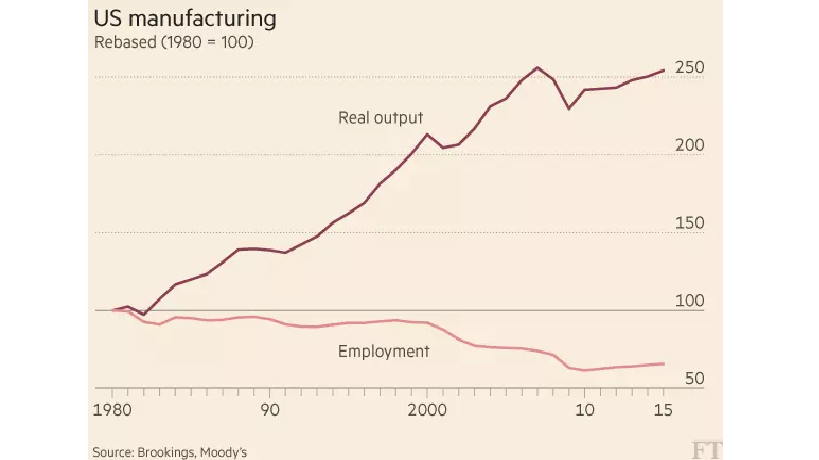
\includegraphics[width=0.80\textwidth]
{us_manuf.png}
\captionsetup{justification=centering}
\caption{US manufacturing real output and employment from 1980-2015. \\ Output rises despite a fall in employment.}
\label{fig:manufacturing}
\end{center}
\end{figure}

Reich argues that this technological trend, together with the lack of a countervailing force, ``is putting more and more value in fewer and fewer hands while reducing the real wages of most...[We] are lurching toward a capitalism so top-heavy it cannot be sustained'' \cite[Reich 214]{Reich}. Without a means of sharing the increasing rewards from technology that otherwise go toward few wealthy individuals, the middle class will vanish. With their disappearance, the well from which the corporation draws its economic power evaporates. The corporation then crumbles and the economic institution tumbles over the cliff's edge. 

The political institution, whose success is intimately connected with the well-being of the economic institution, must introduce a countervailing force. However, a political response alone is not enough to stop the momentum. We make the argument that there must be an \linebreak \textit{inertial} change from the elements within the matrix of the economic institution. In particular, the corporation must realign itself to address the pressing issue of growing income inequality. One solution lies within a fundamental shift from shareholder-centered governance to stakeholder-centered governance. With this inertial change, any countervailing forces imposed by the political institution will be better able to stop the ill-fated momentum of the economic institution. 

\section{\large The Argument for Shareholder-centered Corporate Governance}
We begin by defining several important concepts. We define stakeholders as any party affected by the practices of a corporation. Such parties include the corporation's shareholders, employees, customers, and surrounding communities. The shareholder model of corporate governance is centered on the idea that shareholders are the most important stakeholder, and the primary goal of the corporation is to maximize shareholder wealth. From the shareholder perspective, we define corporate governance as the way in which shareholders assure themselves of getting a return on investment.

\noindent Nobel laureate Milton Friedman writes:
\SetBlockThreshold{1}
\blockquote{There is one and only one social responsibility of business - to use its resources and engage in activities designed to increase its profits so long as it stays within the rules of the game, which is to say, engages in open and free competition without deception or fraud \cite[Friedman 6]{Friedman}.}
Advocates of the shareholder model agree with Friedman in his claim that having this single goal is the most efficient and responsible way to govern a corporation. The general argument is that a well-defined goal of profit maximization promotes the survival of the corporation by making it more competitive, and by helping managers effectively allocate scarce resources. In addition, the need for investors to monitor the company's performance helps create transparency. 

A well-known critique of shareholder theory is that it is ``geared toward short-term profit maximization at the expense of the long-run'' (qtd. in \cite[Danielson \textit{et al}. 2]{Danielson}). However, Danielson \textit{et al}. argue, ``the shareholder model - when viewed from a long-term perspective - provides a better framework than stakeholder theory'' \cite[Danielson \textit{et al}. 2]{Danielson}. They argue that investing in all positive net present value (NPV) projects, regardless of duration\footnote{By this, we mean the time it takes for the NPV project to be reflected in the stock price.}, benefits not only shareholders, but also other stakeholders in current and future timeframes. In particular, positive NPV projects will yield economic benefits for employees and customers. However, a critical failure of Danielson's argument is an assumption that the future state of the economic institution will resemble the current one. By advocating for investments in all positive NPV projects, they assume an unchanging amount of economic power in the consumer base. If the economic power of the middle class evaporates as outlined in our introduction, long-term positive NPV projects may create a bubble in current stock prices. When investors realize the projects fail to meet expectations, the resulting crash will be detrimental to both investors and other stakeholders. Even if viewed from the long-term perspective presented by Danielson \textit{et al}., shareholder-centered corporate governance fails to address the pressing issue of inequality in the economic institution. In fact, unrestrained investment in positive NPV projects may even deepen the impact of technology on unemployment, further decreasing the economic power of the middle class. 
\section{\large The Argument for Stakeholder-centered Corporate Governance}
From the stakeholder-centered perspective, we use the definition of corporate governance as the design of institutions that forces management to internalize the welfare of stakeholders \cite[Garcia-Castro \textit{et al}. 259]{GarciaCastro}.  In such a governance model, managers are pushed to explore beyond the traditional interest group of shareholders in order to understand stakeholder needs, expectations, and values. 

A critique of stakeholder-centered governance is that the allocation of economic surplus to stakeholders (for example, to employees in the form of higher wages) only benefits stakeholders in the short-term. In addition, such policies are claimed to hurt shareholders and adversely affect long-term stakeholder interests, such as job security during turbulent financial times \cite[Danielson \textit{et al}. 4]{Danielson}. However, a study by Ayuso \textit{et al}. shows that high stakeholder engagement at the board level has a statistically significant ($p < 0.05$) and positive effect on financial performance \cite[Ayuso \textit{et al}. 425]{Ayuso}. Contrary to the claims of proponents of shareholder-centered governance theory, it appears that a strong positive relationship exists between stakeholder-centered governance boards and firm financial performance. An attempt at refuting Danielson \textit{et al}.'s second critique was conducted by Garcia-Castro \textit{et al}. who hypothesize that:
\blockquote{Stakeholder centered firms show lower levels of labor turnover and layoffs and have stronger worker displacement policies, higher levels of firm-specific training for employees, higher employee-firm fit, and higher internal knowledge sharing and joint organizational learning among employees than shareholder-centered firms \cite[Garcia-Castro \textit{et al}. 265]{GarciaCastro}.}
The study showed lower turnover, higher firm-specific training, employee-firm fit, knowledge sharing, and learning in firms with stakeholder-centered governance at a statistically significant level ($p < 0.01$). Although layoff rates were lower in stakeholder-centered firms, the difference was not statically significant.  As a result, we acknowledge that a shifting from a shareholder-centered governance structure to a stakeholder-centered governance structure may not fully address the issue of job loss due to technological change. 
\section{\large Addressing Income Inequality}
In \textit{Saving Capitalism}, Robert Reich presents the following idea:
\blockquote{With effective countervailing power, the American corporation could be reimagined and reinvented... The legal privileges of incorporation in America ... would be available only to entities that share the gains from growth with their workers while also taking the interests of their communities and environment into account \cite[Reich 202]{Reich}.}
Reich's reimaged and reinvented corporation seems to be one that follows the stakeholder-centered corporate governance structure as outlined in the preceding section. Indeed, Reich calls upon the example of codetermination in Germany. In the German corporate governance system, management boards oversee day-to-day operations and supervisory boards, in which employees have significant representation, make high-level decisions. The result is ``a higher median wage and a far more secure and prosperous working class than in the United States'' \cite[Reich 202]{Reich}. 

We wished to use simple descriptive statistics to investigate if income inequality is systematically higher in countries with shareholder-centered corporate governance laws than in countries with stakeholder-centered governance laws. To this end, we refer to the classification of countries according to their governance system as developed by La Porta and Garcia-Castro \textit{et al}. (table 1, from \cite[Garcia-Castro \textit{et al}. 268]{GarciaCastro}). 
\begin{figure}[!htbp]
\begin{center}
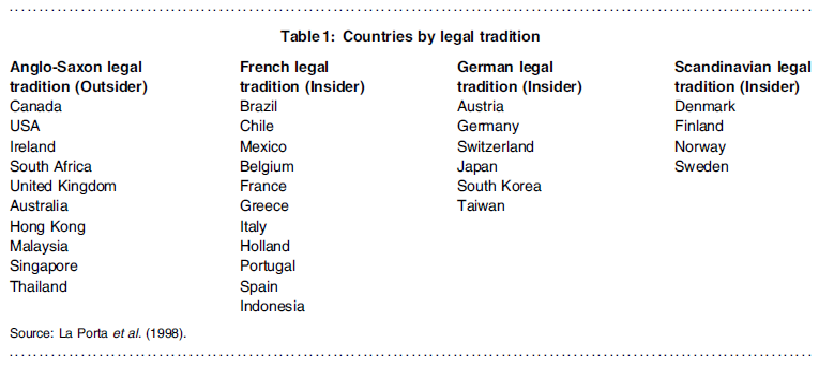
\includegraphics[width=1\textwidth]
{table.png}
\captionsetup{justification=centering}
\end{center}
\end{figure}

As Garcia-Castro \textit{et al}. describe, countries with German legal tradition are broadly defined as stakeholder-oriented industrial systems. For example, most German and Austrian firms have adopted employment standards consistent with the ones described by stakeholder-centered governance theory \cite[Garcia-Castro \textit{et al}. 268]{GarciaCastro}. On the other hand, Anglo-Saxon legal tradition favors a shareholder-centered corporate governance model. Countries following the French and Scandinavian legal tradition are more difficult to classify as purely stakeholder or shareholder economies. For this reason, we omit their results from the primary discussion and leave them for the reader in the appendix. 

Using data from the United Nations Development Programme's \textit{Human Development Report} (2009) and La Porta's country classification, we tabulated each country's ratio of the average income of the richest $10\%$ to the poorest $10\%$ (denoted $10\% \text{ }R/P$). A $10\% \text{ } R/P$ value of $1$ signifies perfect equality. Higher values signify greater inequality. Using the data for countries in La Porta's classification, we found average $10\% \text{ }R/P$ for countries following the Anglo-Saxon (shareholder) legal tradition to be $16.4 \pm 7.1$. On the other hand, the average $10\% \text{ }R/P$ for countries following the German (stakeholder) legal tradition is $6.9 \pm 1.5$. The reported uncertainty represents one (sample) standard deviation. At this uncertainty, the intervals do not overlap, hinting to a possible systematic bias in which countries that follow shareholder-centered corporate governance tend to have greater income inequality. One weakness of La Porta's classification is that it does not include all countries. Using the limited data, we attempt a rough approximation of the shape of the true distribution of countries falling into the German and Anglo-Saxon classifications using Gaussian distributions centered at the sample mean and truncated at $1$. 
\begin{figure}[!htbp]
\begin{center}
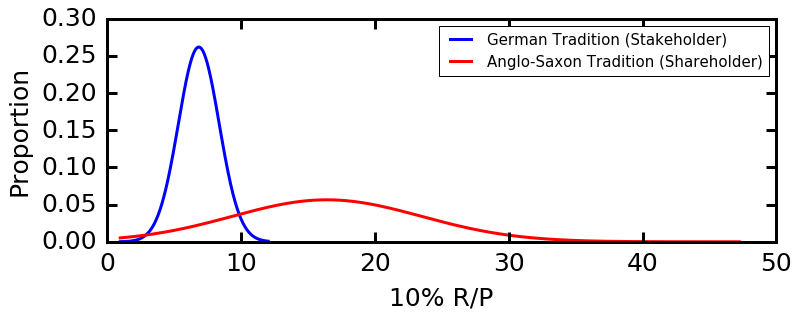
\includegraphics[width=.90\textwidth]
{un10rp.png}
\captionsetup{justification=centering}
\caption{Expected proportion of countries in the German (resp. Anglo-Saxon) classification at a given $10\% \text{ } R/P$ value.}
\end{center}
\end{figure}

In addition to including more countries, a more sophisticated study could develop a scale to assess the degree to which a particular country's governance tradition is shareholder-centered or stakeholder-centered. One could then perform a regression using this scale as an independent variable against each country's $10\% \text{ } R/P$. Such a study might be able to confirm a correlation between the type of corporate governance and the degree of inequality in the country. 

We have shown a potential relationship between corporate governance and income inequality. In the next section, we discuss what type of countervailing measures might be appropriate to stop the economic institution's ill-fated momentum.

\section{\large Countervailing Forces}
As we have discussed in the introduction, a countervailing force to stop the ill-fated momentum of the economic institution must come from the realm politics. However, since those with the most economic power have so deeply institutionalized politics, any proposed countervailing force will be unlikely to change the status quo. Robert Reich mentions an example of a bill that would have acted as a strong countervailing force in reversing the inequality trend. The bill introduced in the California legislature would have tied corporate tax to the ratio of CEO to median worker pay. He argues that the bill would have led to the creation of jobs by increasing the capacity of people to buy, thus giving reason for companies to expand and hire \cite[Reich 197]{Reich}. Despite this, the California Chamber of Commerce dubbed the bill as a ``job killer,'' and the bill was subsequently rejected in 2014 \cite[CBS/AP]{CBS}. Because of the difficulty in passing mandatory compliance standards through a political process, we wish to evaluate the effectiveness of non-mandatory governance codes, which may come from the government, NGOs, or professional associations.

In a study of Russian firms, Okhmatovskiy and David argue that organizations often develop their own corporate governance standards in response to non-mandatory external standards. The effectiveness of these governance standards is dependent on the influence of the firm's shareholders who value good corporate governance. In particular, they argue, ``factors that decrease firms' dependence on minority shareholders increase the probability of a ceremonial [internal governance code]'' \cite[Okhmatovskiy and David 170]{David}. We wish to extend this notion to firms in shareholder-centered countries (while acknowledging the limitations of such an extension without empirical evidence). We make the argument that non-mandatory external standards will lead to the adoption of ceremonial governance codes unless the firm's shareholders are representative of its stakeholders. In other words, unless stakeholders have adequate board representation, external standards will have little effect. As a result, the corporation will continue to pursue the best interests of its shareholders, doing little to address widening income inequality.  

\section{\large Conclusion}
The current trend of widening income inequality is not sustainable for the economic institution. To save the corporation and the encapsulating economic institution, a countervailing force is necessary. However, if one accepts Roy's three propositions, there exists significant difficulty in enacting the required compulsory countervailing forces in countries where shareholder-centered governance is prevalent. The relatively low inequality in stakeholder-centered countries hints toward a hope that lies in reprioritizing corporate governance. This amounts to making the corporation's shareholders more representative of its stakeholders and subsequently adopting a more stakeholder-centered governance model. In such a scenario, corporations will be inclined to closely follow externally imposed codes and move in a direction to reverse the trend of growing inequality. 
\pagebreak
\bibliographystyle{IEEEtran}
\bibliography{MyBibliography.bib}
\newpage
\appendix

\section{Data Tables}
Data sourced from the United Nations Development Programme's \textit{Human Development Report: Overcoming Barriers: Human Mobility and Development} (2009).
\begin{table}[htbp!]
	\caption{Anglo-Saxon legal tradition}
	\centering
		\begin{tabular}{ccc}
			\textbf{Country} & $\mathbf{10\% \text{ } R/P}$ &\\
			  \hline
			Canada&$9.4$\\
			USA&$15.9$\\
			Ireland&$9.4$\\
			South Africa&$33.1$\\
			Australia&$13.8$\\
            Hong Kong&$12.5$\\
            Malaysia&$17.8$\\
            Singapore&$22.1$\\
            Thailand&$12.6$\\
            \hline
            \textbf{Mean}&$\mathbf{16.4}$\\
            \textbf{Standard Deviation}&$\mathbf{7.1}$\\
			\hline
            $ $ & $ $ \\
            $ $ & $ $ \\
            $ $ & $ $ 
		\end{tabular}
\end{table}

\begin{table}[htbp!]
	\caption{French Legal Tradition}
	\centering
		\begin{tabular}{ccc}
			\textbf{Country} & $\mathbf{10\% \text{ } R/P}$ &\\
			  \hline
			Brazil&$25.0$\\
			Chile&$26.2$\\
			Mexico&$21.6$\\
			Belgium&$8.2$\\
			France&$9.1$\\
            Greece&$10.2$\\
            Italy&$11.6$\\
            Holland&$9.2$\\
            Portugal&$15.0$\\
            Spain&$10.3$\\
            Indonesia&$7.8$\\
            \hline
            \textbf{Mean}&$\mathbf{14.0}$\\
            \textbf{Standard Deviation}&$\mathbf{6.9}$\\
			\hline
		\end{tabular}
\end{table}

\pagebreak

\begin{table}[htbp!]
	\caption{German legal tradition}
	\centering
		\begin{tabular}{ccc}
			\textbf{Country} & $\mathbf{10\% \text{ } R/P}$ &\\
			  \hline
			Austria&$6.9$\\
			Germany&$6.9$\\
			Switzerland&$9.0$\\
			Japan&$4.5$\\
			South Korea&$7.8$\\
            Taiwan&$6.1$\\
            \hline
            \textbf{Mean}&$\mathbf{6.9}$\\
            \textbf{Standard Deviation}&$\mathbf{1.5}$\\
			\hline
            $ $ & $ $ \\
            $ $ & $ $ \\
            $ $ & $ $ 
		\end{tabular}
\end{table}

\begin{table}[htbp!]
	\caption{Scandinavian Legal Tradition}
	\centering
		\begin{tabular}{ccc}
			\textbf{Country} & $\mathbf{10\% \text{ } R/P}$ &\\
			  \hline
			Denmark&$8.1$\\
			Finland&$5.6$\\
			Norway&$6.1$\\
			Sweden&$6.2$\\
            \hline
            \textbf{Mean}&$\mathbf{6.5}$\\
            \textbf{Standard Deviation}&$\mathbf{1.1}$\\
			\hline
		\end{tabular}
\end{table}

\newcommand\blfootnote[1]{%
  \begingroup
  \renewcommand\thefootnote{}\footnote{#1}%
  \addtocounter{footnote}{-1}%
  \endgroup
}

\blfootnote{
\textit{E-mail address}, D. Hutama: \quad \href{mailto:daniel.hutama@mail.mcgill.ca}{daniel.hutama@mail.mcgill.ca}}

\end{document}
%%%%%%